Opisani sustav svoju primjenu bi mogao naći u raznim situacijama: od ispravljanja ručno zapisanih odgovora na ispitu, do samog podsustava u sustavu za očitavanja rukom pisanoga teksta. U sklopu ovog projekta isprobana je integracija navedenoga sustava na mobilni uređaj \emph{Apple iPhone} sa zaslonom osjetljivim na dodir, gdje bi korisnik unosio tekst crtanjem slova na samom zaslonu.

\section{Pretvorba modela}

Kako je već spomenuto, za učenje klasifikatora konvolucijske neuronske mreže korišten je radni okvir \emph{Keras}. Navedeni okvir omogućava izlučivanje naučenoga modela i njegovih težina koji se kasnije mogu upotrebljavati u drugim radnim okvirima i programskim jezicima.

Jedan takav okvir je i \emph{Apple-ov} \emph{Core ML} \cite{coreml}. Navedeni okvir omogućava uključivanje i uporabu naučenih modela iz raznih okvira, poput \emph{Keras}, \emph{Xgboost}, \emph{scikit-learn} i drugih, na \emph{Apple-ovim} uređajima, što uključuje širok spektar: od pametnih satova, preko mobilnih uređaja do osobnih računala.

Posebnost navedenoga okvira je što se naučeni modeli nalaze na uređaju te su optimirani za izvođenje na prijenosnim uređajima gdje potrošnja energije i resursa mora biti što manja.

Radni okvir \emph{Core ML} je pisan u programskom jeziku \emph{Swift} te u pozadini koristi sljdeće radne okvire:
\begin{itemize}
  \item \emph{Accelerate} - optimirane matrične i vektorske operacije
  \item \emph{BNNS} - skup funkcija za lakše implementiranje neuronskih mreža
  \item \emph{Metal Performance Shaders} - izvođenje računskih operacija na \emph{GPU-u}
\end{itemize}

Postupak pretvorbe \emph{Keras} modela se obavljao koristeći službeni \emph{Appleov} alat \emph{coremltools} pisan u programskom jeziku \emph{Python}. Program kao parametar prima opis modela u definiranom \emph{JSON} formatu i njegove težine, te na izlazu vraća \emph{ML model} koji se zatim može koristiti na \emph{Appleovim} \emph{iOS} i \emph{macOS} sustavima.

\section{Aplikacija}

Za potrebe ovog rada napisana je aplikacija imena \emph{SmartLetter} u programskom jeziku \emph{Swift}. Grafičko sučelje navedene aplikacije prikazano je na slici \ref{fig:app}. Korisnik dodirom i potezima crta slovo na platnu te aplikacija ispisuje prepoznato slovo. Samo prepoznavanje znaka traje ispod jedne milisekunde, a to obuhvaća: pretprocesiranje ulaznog znaka (izvlačenje okvira, centriranje i skaliranje), pretvorba u crno-bijelu sliku, propuštanje kroz konvolucijsku neuronsku mrežu te na kraju obradu izlaza mreže, to jest ispis prepoznatog znaka.

\begin{figure}[htb]
    \centering
    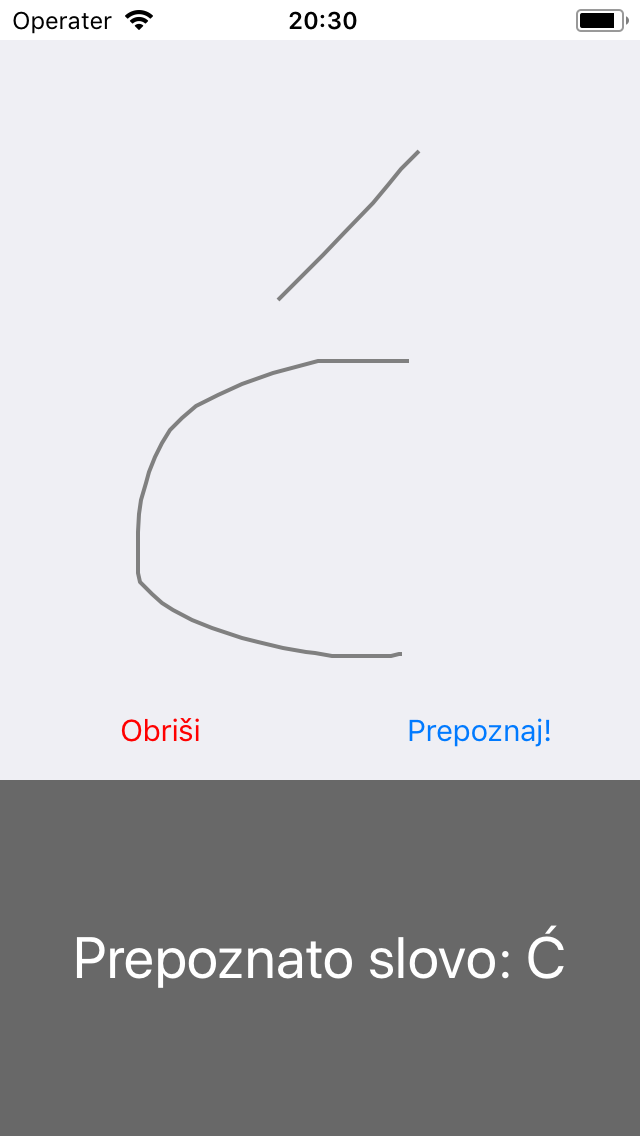
\includegraphics[width=6cm]{images/app2.png}
    \caption{\emph{SmartLetter} aplikacija.}
    \label{fig:app}
\end{figure}

Kako sama aplikacija i nema neku svrhu osim isprobavanja sustava za prepoznavanje znakova, implementirana je dodatna komponenta aplikacije, to jest tipkovnica koja se može koristiti kroz cijeli \emph{iOS} sustav. Tipkovnica i primjer korištenja je prikazan na slici \ref{fig:keyboard}. Korisnik unosi tekst crtanjem na platnu. S lijeve strane je dugme za izmjenu velikih i malih slova, jer kako je već napomenuto, sustav na izlazu ima $32$ razreda, to jest združena pojedina velika i mala slova proširene hrvatske abecede. Na desnoj strani je dugme za brisanje prethodno napisanoga slova te prelazak u novi red. Za sam razmak se koristi posebni znak crtice "-".

Kako bi unos teksta bio što brži, ne koristi se posebno dugme za prepoznavanje već se prati kad je korisnik završio s crtanjem, to jest podignuo prst sa zaslona te se zatim vrši prepoznavanje. Navedeni pristup ima problem kod znakova koji su sastavljeni od više odvojenih dijelova, poput znakova č, ć, ž i sličnih jer korisnik mora podići prst kako bi nacrtao drugi dio znaka. Kao riješenje implementirana je odgoda prepoznavanja gdje sama aplikacija čeka određeno vrijeme idući unos, te ukoliko se ne dogodi tek onda vrši prepoznavanje znaka, a ako se dogodi onda samo nastavi iscrtavanje na već prije iscrtani znak. Isprobano je više intervala čekanja, no to uvelike ovisi o samo korisniku i njegovoj spretnosti prilikom pisanja. Najbolje vrijeme čekanja isprobanih na nekolicini korisnika je ispalo između $300$ i $600$ milisekundi.

\begin{figure}[htb]
    \centering
    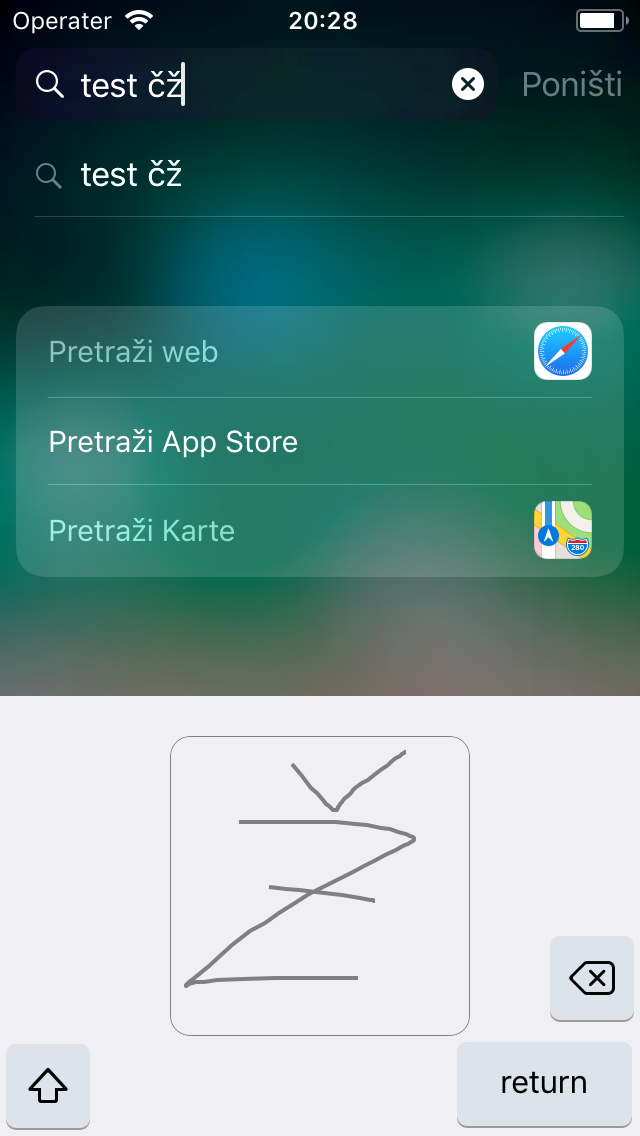
\includegraphics[width=6cm]{images/app1.png}
    \caption{\emph{SmartLetter} tipkovnica u sustavu \emph{iOS}.}
    \label{fig:keyboard}
\end{figure}

